\begin{figure*}[!t]
    \centering
    % \vspace{-0.2cm}
    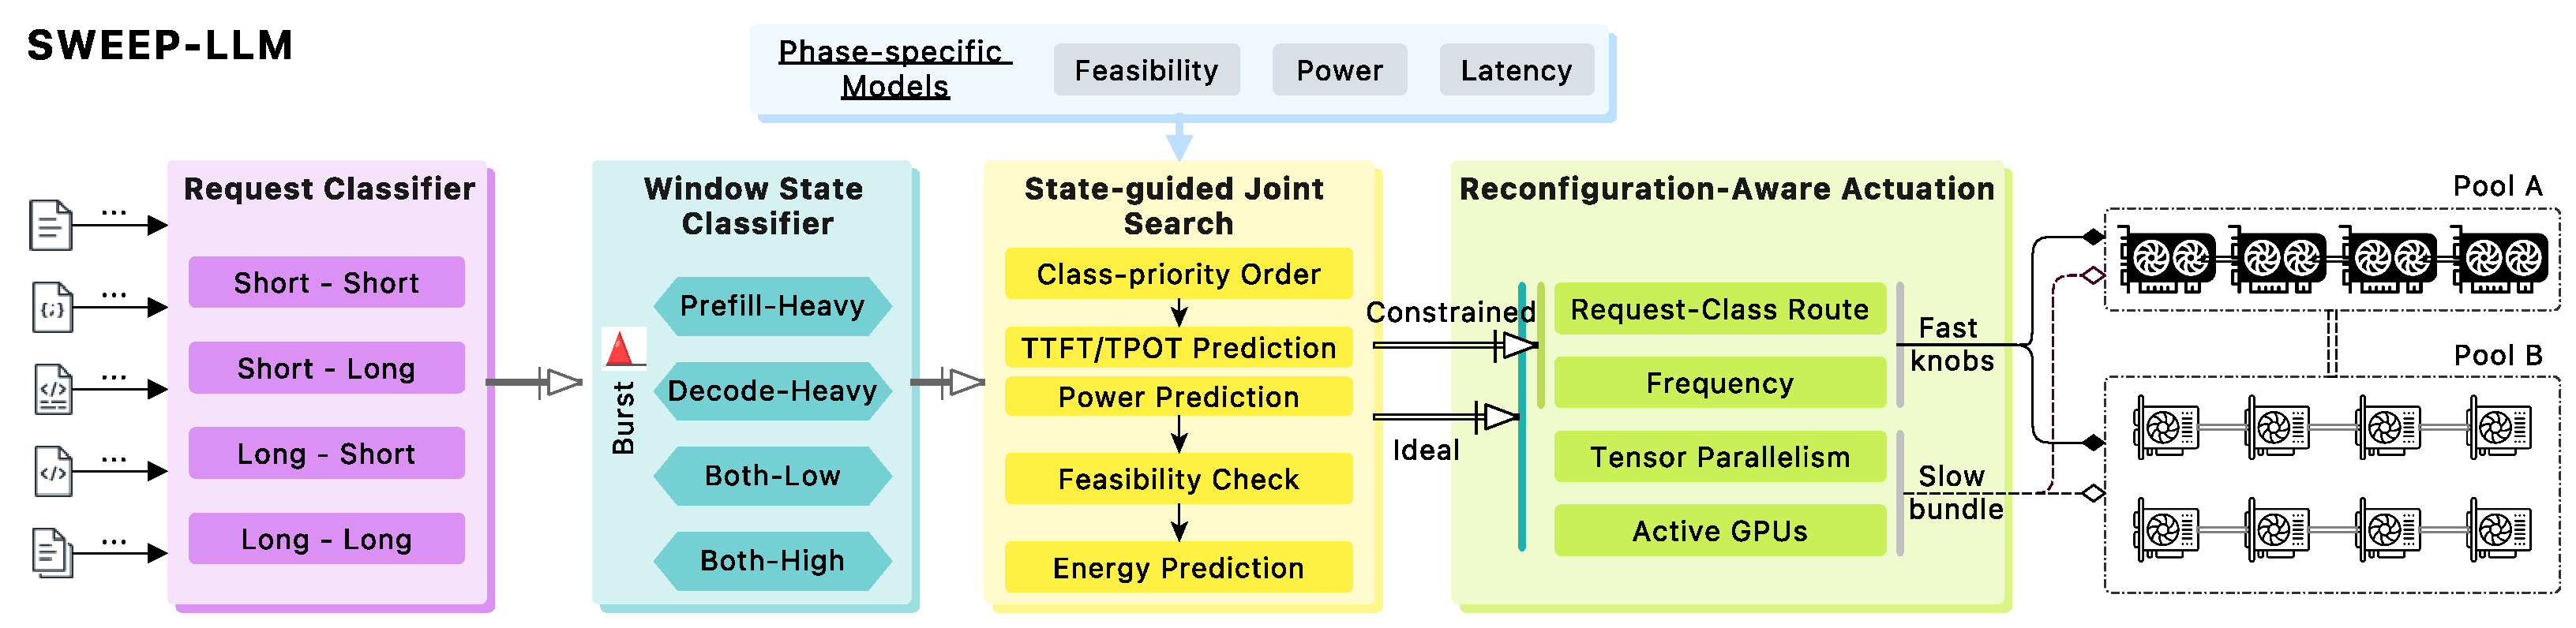
\includegraphics[width=\textwidth]{./figures/overview.eps}
    % \vspace{-0.5cm}
    \caption{Overview of the proposed energy-aware scheduling framework.}
    % \vspace{-0.2cm}
    \label{fig:overview}
\end{figure*}


\section{SWEEP-LLM Design}
\label{sec:design}

% This section presents the runtime design of SWEEP-LLM for energy-efficient LLM inference on heterogeneous, phase-disaggregated GPU clusters. SWEEP-LLM jointly optimizes four coupled control dimensions: class-aware routing, tensor parallelism, GPU frequency, and GPU allocation. Its design is shaped by four requirements: the scheduler must capture request heterogeneity within each window, adapt to changing workload states across windows, search a large coupled configuration space efficiently, and account for the fact that different controls incur very different reconfiguration costs.
% This section presents the runtime design of SWEEP-LLM for energy-efficient LLM inference on heterogeneous, phase-disaggregated GPU clusters.
This section presents the runtime design of SWEEP-LLM.
%  for energy-efficient LLM inference on heterogeneous, phase-disaggregated GPU clusters.
% The design is organized around four practical considerations: capturing request heterogeneity within each window, adapting to changing workload states across windows, searching a large coupled configuration space efficiently, and accounting for the fact that different controls incur very different reconfiguration costs.
It is organized around four requirements: capturing request heterogeneity within each window, estimating the phase bottleneck for the window, searching the coupled configuration space efficiently, and accounting for the fact that different controls incur different reconfiguration costs.
% This section presents the runtime design of SWEEP-LLM. The scheduler jointly controls four coupled decisions---per-class phase routing, tensor parallelism, GPU frequency, and active GPU allocation---while respecting that these controls operate at different timescales. 
% It is organized around four questions: how to represent heterogeneous requests within a window, how to identify the current phase bottleneck, how to search the coupled configuration space efficiently, and how to apply slow reconfigurations without excessive churn.


% OLD OVERVIEW TEXT
% We consider a heterogeneous serving cluster with two GPU pools, denoted pool~A and pool~B, containing $G_A$ and $G_B$ GPUs, respectively.
% Each request consists of a prefill phase and a decode phase, and the two phases may execute on different pools.
% If they do, the request incurs cross-pool KV-cache transfer overhead, which SWEEP-LLM accounts for explicitly during route-dependent latency and energy evaluation.
% SWEEP-LLM routes requests at request-class granularity, allowing different request classes within the same scheduling window to take different routes.
% Each incoming request is mapped to one of $K$ classes according to its input and output lengths (\S\ref{sec:request_classes}).
% For each class $c \in \{1,\ldots,K\}$, the scheduler assigns one deterministic route
% $r\_c \in \{A\!\to\!A, A\!\to\!B, B\!\to\!A, B\!\to\!B\}$.
% The full configuration optimized at each scheduling window is
% SWEEP-LLM operates over scheduling windows of duration $W$.
% For each window, the workload is summarized by the aggregate arrival rate $\lambda$ and the per-class statistics $\{\pi_c,\tilde{\mathrm{il}}_c,\tilde{\mathrm{ol}}_c\}_{c=1}^{K}$, where $\pi_c$ is the class fraction and $\tilde{\mathrm{il}}_c$ and $\tilde{\mathrm{ol}}_c$ are representative input and output lengths for class $c$.
% The aggregate prefill and decode token demands are
% The scheduler selects the minimum-energy configuration subject to latency constraints on every active request class:
% Here $\widehat{\mathrm{TTFT}}_c$ and $\widehat{\mathrm{TPOT}}_c$ are the predicted latencies for class~$c$ under its assigned route, computed using the models in \S\ref{sec:phase_a_models}.
% Candidates that violate the latency constraint of any active class are discarded immediately.

% ---------------------------------------------------------------
\subsection{Overview}
\label{sec:overview}
% ---------------------------------------------------------------

% Figure~\ref{fig:overview} summarizes the runtime workflow of SWEEP-LLM.
% The scheduler operates over windows of duration $W$ and seeks the lowest-energy configuration that satisfies TTFT and TPOT constraints on a heterogeneous, phase-disaggregated cluster.
% We consider two GPU pools, denoted pool~A and pool~B, containing $G_A$ and $G_B$ GPUs, respectively.
% Each request consists of a prefill phase and a decode phase, and the two phases may execute on different pools.
% If they do, the request incurs cross-pool KV-cache transfer overhead, which SWEEP-LLM accounts for explicitly during route-dependent latency and energy evaluation.

Figure~\ref{fig:overview} summarizes the runtime workflow.
SWEEP-LLM targets a heterogeneous, phase-disaggregated cluster with two GPU pools, denoted A and B.
Pool $k\in\{A,B\}$ contains $G_k$ GPUs.
Each request has a prefill phase and a decode phase, and the two phases may run on the same pool or on different pools.
% When they run on different pools, the KV cache produced by prefill must be transferred to the decode pool, and SWEEP-LLM includes this route-dependent transfer cost when estimating latency.
% Cross-pool routes additionally incur a KV-cache transfer cost, which SWEEP-LLM charges as a route-dependent latency term (\S\ref{sec:phase_a_models}).
SWEEP-LLM makes decisions at scheduling boundaries.
At each boundary, it estimates the workload for the next control window from recent traffic statistics, or from a deployment-provided short-horizon forecast when available.
Based on this estimate, SWEEP-LLM searches over four coupled control dimensions: per-class routing, tensor parallelism, GPU frequency, and active GPU allocation for prefill and decode.
Requests are grouped into $K$ classes, indexed by $c\in\{1,\ldots,K\}$.
For each class $c$, the scheduler may choose any route $r_c \in \{A\!\to\!A, A\!\to\!B, B\!\to\!A, B\!\to\!B\}$.
The complete configuration considered by the search is
\begin{equation}
\mathcal{C} =
\bigl(
r_1,\ldots,r_K,\;
f_A,f_B,\;
\mathrm{TP}_A,\mathrm{TP}_B,\;
n_{A,\mathrm{pf}},n_{A,\mathrm{dc}},\;
n_{B,\mathrm{pf}},n_{B,\mathrm{dc}}
\bigr),
\label{eq:config}
\end{equation}
where $f_k$ is the GPU frequency of pool $k$, $\mathrm{TP}_k$ is its tensor-parallel degree, and $n_{k,\mathrm{pf}}$ and $n_{k,\mathrm{dc}}$ are the active GPUs assigned to prefill and decode.
A candidate is valid only if each pool uses no more GPUs than it contains and each prefill/decode allocation can be partitioned into whole TP groups:
\begin{equation}
n_{k,\mathrm{pf}} + n_{k,\mathrm{dc}} \le G_k,
\qquad
n_{k,\mathrm{pf}},n_{k,\mathrm{dc}} \equiv 0 \pmod{\mathrm{TP}_k}.
\label{eq:gpu_alloc_constraint}
\end{equation}
% NEW: reviewer-proofing design-choice note --- one TP degree per pool (vs.\ per-phase TP).
We use one tensor-parallel degree and one GPU frequency per pool, rather than separate per-phase TP degrees or per-GPU frequencies, to keep each pool's serving layout homogeneous.
With a fixed $\mathrm{TP}_k$, changing $n_{k,\mathrm{pf}}$ and $n_{k,\mathrm{dc}}$ reallocates whole TP groups between phases without introducing different model-partition layouts within the same pool.
Using one frequency $f_k$ per pool similarly avoids per-GPU DVFS skew within a TP group and keeps the runtime actuation and power model at the pool level.
Phase specialization is still captured through hardware-aware routing across pools and through separate prefill/decode capacity allocations.
% The joint search space induced by Eq.~\ref{eq:config} is large because routing, TP, active GPU allocation, and frequency interact through pool load, KV-transfer overhead, service capacity, and power.

SWEEP-LLM evaluates each candidate with the predictive models from \S\ref{sec:phase_a_models} and selects the lowest-energy feasible configuration:
\begin{equation}
\min_{\mathcal{C}} \; E_{\mathrm{window}}(\mathcal{C})
\quad \text{s.t.} \quad
\forall c:\;
\begin{cases}
\widehat{\mathrm{TTFT}}_c(\mathcal{C}) \le \mathrm{SLO}_{\mathrm{TTFT}}, \\
\widehat{\mathrm{TPOT}}_c(\mathcal{C}) \le \mathrm{SLO}_{\mathrm{TPOT}}.
\end{cases}
\label{eq:objective}
\end{equation}
The framework comprises four components.

\subsubsection*{\textnormal{\textbf{\circlednum{1}: Request Classification (\S\ref{sec:request_classes})}}}
% A control window may contain requests with very different prompt lengths and generation demands, so assigning one route to all requests in the window is too coarse. 
% SWEEP-LLM therefore groups arriving requests into $K$ classes using information available at admission: the known input length and an estimated output length. 
% SWEEP-LLM uses $K=4$ classes, corresponding to long/short prompt length crossed with long/short estimated output length. 
% The scheduler then chooses one route per class, allowing different token profiles in the same control window to use different prefill/decode placements.

A control window may contain requests with very different prompt lengths and generation demands, so assigning one route to all requests in the window is too coarse.
SWEEP-LLM therefore groups requests into a small number of token-length classes using information available at admission, and chooses one route per class.
This lets different token profiles in the same control window use different prefill/decode placements; \S\ref{sec:request_classes} defines the class taxonomy.

\subsubsection*{\textnormal{\textbf{\circlednum{2}: Workload Classification (\S\ref{sec:window_classifier})}}}
% OLD (condensed; the per-class statistics and the aggregate-demand equation are moved to \S\ref{sec:window_classifier}, where they are used):
% After request classification, SWEEP-LLM summarizes the estimated workload for the next control window.
% The summary includes the expected arrival rate $\lambda$ and per-class statistics $\{\pi_c,\tilde{\mathrm{il}}_c,\tilde{\mathrm{ol}}_c\}_{c=1}^{K}$.
% Here, $\pi_c$ is the expected fraction of requests in class $c$, and $\tilde{\mathrm{il}}_c$ and $\tilde{\mathrm{ol}}_c$ are representative input and estimated output lengths for that class.
% From these statistics, the scheduler computes aggregate prefill and decode token demand,
% \begin{equation}
% D_{\mathrm{pf}} = \lambda \sum_{c=1}^{K} \pi_c \tilde{\mathrm{il}}_c,
% \qquad
% D_{\mathrm{dc}} = \lambda \sum_{c=1}^{K} \pi_c \tilde{\mathrm{ol}}_c.
% \end{equation}
% SWEEP-LLM uses this demand summary to assign the upcoming window to one of four coarse bottleneck states: ...
After request classification, SWEEP-LLM summarizes the estimated workload for the next control window into aggregate prefill and decode demand.
It uses this demand summary to assign the upcoming window to one of four coarse bottleneck states: \textsc{Prefill\_Heavy}, \textsc{Decode\_Heavy}, \textsc{Both\_Low}, or \textsc{Both\_Heavy}.
It also tracks a \textsc{Burst} flag when recent traffic indicates a sharp load increase.
The state label and burst flag do not determine the final routes or resource allocation directly. 
Instead, they guide how the subsequent joint search generates and orders candidates.

\subsubsection*{\textnormal{\textbf{\circlednum{3}: State-Specific Joint Search (\S\ref{sec:joint_search})}}}
% Given the request classes and the current window state, SWEEP-LLM jointly considers four control dimensions: (i) per-class routing, (ii) tensor parallelism (TP), (iii) GPU frequency, and (iv) active GPU allocation for prefill and decode.
% For each class $c$, routing is chosen as one deterministic route $r_c \in \{A\!\to\!A, A\!\to\!B, B\!\to\!A, B\!\to\!B\}$, and the full window-level configuration is
% Given the request classes and the predicted bottleneck state, 

Searching all combinations in Eq.~\ref{eq:config} every window would be expensive.
% OLD: SWEEP-LLM therefore uses the bottleneck state to prioritize the most relevant parts of the search space.
% OLD: The state determines which pool-level candidates are considered first, which class order is used when enumerating route assignments, and which anchor configurations seed the search.
SWEEP-LLM therefore uses the bottleneck state to decide which pool-level candidates and anchor route maps to examine first, and in what class order to assign routes.
% Each state selects a pool-candidate set, a class-priority order, and seeded anchor configurations, while the objective and the admissible route set remain common across states.
% Each state selects which pool-level candidates to explore first, which class order to use during route enumeration, and which anchor configurations to seed.
% The state does not preassign routes to classes or change the energy/latency objective.
% Final routes and resource allocations are still selected by the model-based optimization.
% OLD (condensed; the formal two-search definition now lives only in \S\ref{sec:joint_search}):
% SWEEP-LLM performs two searches with different scopes.
% The constrained search keeps the currently deployed TP degrees and active-GPU allocations fixed, and re-optimizes the fast controls: per-class routing and GPU frequency.
% This search produces the best configuration that can be applied without changing the deployed serving instances.
% The ideal search allows all variables in Eq.~\ref{eq:config} to vary, and therefore identifies the best target configuration under the current workload estimate.
% Because the ideal search may require slow reconfiguration, its result is passed to the actuation logic described next.
% OLD (condensed to one sentence; detail deferred to \S\ref{sec:joint_search} and the actuation handoff to component 4 / \S\ref{sec:reconfig}):
% SWEEP-LLM runs two searches: a constrained search that re-optimizes only the fast controls (routing and frequency) under the deployed bundles, and an ideal search that frees all variables for the estimated next-window workload.
% The constrained result gives the immediately deployable operating point, while the ideal result is a target that may require slow reconfiguration and is therefore passed to the actuation logic (\S\ref{sec:reconfig}); the two searches are formalized in \S\ref{sec:joint_search}.
It then runs a constrained search for immediately deployable routing and frequency decisions, and an ideal search for slow-bundle targets; \S\ref{sec:joint_search} formalizes both searches.

% SWEEP-LLM runs two related searches.
% The constrained search keeps the currently deployed slow controls fixed and re-optimizes the fast controls, routing and frequency, to find the best configuration that can be applied immediately.
% The ideal search frees all variables in Eq.~\ref{eq:config} and identifies the best full configuration, but it is executed only on cold start, on a sustained state change, on a burst-flag toggle, when the arrival rate or class mix crosses the \textsc{NeedIdealSearch} thresholds, or after a periodic refresh interval.
% The ideal result updates slow-bundle targets rather than being applied immediately.

% Eq.~\ref{eq:objective} is the conceptual feasibility target. In the frozen cross-strategy evaluation (\S\ref{sec:evaluation}), we report feasibility using a common utilization gate ($\rho \le 1$) applied identically to all strategies, rather than thresholding the raw latency regressions; strict SLO-oriented gates are evaluated separately as a sensitivity check.
% Routing and frequency can be changed quickly, whereas TP and active GPU allocation require comparatively expensive actions such as instance restart, model reshaping, or scale operations.
% % SWEEP-LLM therefore combines triggered slow-knob optimization with bundle-stability gating and an emergency override path (\S\ref{sec:reconfig})
% To support fast runtime decisions, SWEEP-LLM separates the joint search into two forms.
% The \emph{constrained search} keeps the currently deployed slow knobs fixed and re-optimizes only routing and frequency.
% It therefore yields the best immediately deployable operating point.
% The \emph{ideal search} frees all variables in Eq.~\ref{eq:config} and identifies the best full configuration, but it is executed only on cold start, on a sustained state change, on a burst-flag toggle, when the arrival rate or class mix crosses the \textsc{NeedIdealSearch} thresholds, or after a periodic refresh interval.
% Both searches use the same objective and feasibility criterion.
% They differ only in the candidate set explored.
% In implementation, the admission rule can be instantiated as the common $\rho$-gate or a stricter classifier/latency gate; the evaluation uses the common $\rho$-gate so that all strategies face the same feasibility standard (\S\ref{sec:eval_setup}).
% % Within each state, the joint search combines three ingredients: a state-specific pool-candidate set, admissible per-class route sets, and a state-dependent class-priority order.
% The search is state-guided rather than globally exhaustive over all control dimensions: each state determines a pool-candidate set, a class-priority order, and seeded anchor configurations; the admissible per-class route set remains the same across states, thereby reducing search cost while preserving one common objective and feasibility criterion.

\subsubsection*{\textnormal{\textbf{\circlednum{4}: Reconfiguration-Aware Execution (\S\ref{sec:reconfig})}}}
% OLD (condensed to a high-level pointer; bundle definition, target/promote mechanism, stability counter, and atomicity now live only in \S\ref{sec:reconfig}):
% SWEEP-LLM separates optimization from actuation because not all control decisions have the same reconfiguration cost.
% Per-class routing and GPU frequency are fast controls.
% They can be updated at each scheduling boundary, so SWEEP-LLM applies them directly from the constrained-search result.
% In contrast, TP degree and active-GPU allocation are slow controls.
% Changing them may require instance restart, model reshaping, or GPU reallocation.
%
% SWEEP-LLM groups the slow controls of each pool into a deployment bundle $\mathbf{b}_k=(\mathrm{TP}_k,n_{k,\mathrm{pf}},n_{k,\mathrm{dc}})$.
% When the ideal search recommends a new bundle, SWEEP-LLM records it as a target rather than applying it immediately.
% A target bundle is promoted to the running system after it remains stable for a configurable number of consecutive windows.
% This policy avoids reconfiguring TP and GPU allocation in response to isolated workload fluctuations.
% It also ensures that TP and active-GPU allocation change together, avoiding transient deployments in which the two decisions are inconsistent.
SWEEP-LLM separates optimization from actuation because routing and frequency can be changed quickly, while TP degree and active-GPU allocation are slower deployment changes.
It applies fast controls from the constrained-search result at each scheduling boundary.
It treats $\mathbf{b}_k=(\mathrm{TP}_k,n_{k,\mathrm{pf}},n_{k,\mathrm{dc}})$ as one slow deployment choice for each pool, and applies a new bundle only after the same target persists across windows.
% \par\noindent 
% Finally, SWEEP-LLM converts the search result into a stable runtime policy.
% Fast knobs, per-class routing and GPU frequency, are applied immediately at every window.
% Slow knobs, TP and active GPU allocation, 
% are represented by the per-pool deployment bundle
% \[
% \mathbf{b}_k=(\mathrm{TP}_k,n_{k,\mathrm{pf}},n_{k,\mathrm{dc}}),
% \]
% and 
% % REMOVED: dangling fragment (subject was commented out above; duplicates the promotion sentence earlier in this component).
% are promoted only when their targets remain stable across consecutive windows.
% If the currently deployed bundles become infeasible but the ideal search finds a feasible alternative, SWEEP-LLM can immediately promote the target bundle through an emergency override.
% This separation allows SWEEP-LLM to compute one joint operating point every window while avoiding unnecessary slow reconfigurations.

% ---------------------------------------------------------------
% \subsection{Design Challenges}
% \label{sec:challenges}
% ---------------------------------------------------------------
%
% SWEEP-LLM is organized around four challenges.
%
% \subsubsection*{\textnormal{Challenge \circlednum{1}: request heterogeneity}}
% A single scheduling window may contain requests with very different input and output lengths. Since the energy-efficient route depends on the phase composition of the request, applying one routing decision to the entire window is too coarse.
%
% \subsubsection*{\textnormal{Challenge \circlednum{2}: workload dynamics}}
% Both the aggregate arrival rate and the relative pressure on prefill and decode can change across adjacent windows. The energy-efficient routing and provisioning policy therefore depends on the current bottleneck structure rather than on request rate alone.
%
% \subsubsection*{\textnormal{Challenge \circlednum{3}: search complexity}}
% The joint search space induced by Eq.~\ref{eq:config} is large. Routing changes pool loads and KV-transfer overhead, TP changes per-instance service capacity, GPU allocation changes concurrency, and frequency changes both latency and power. Exhaustive search is therefore too expensive to run naively in every scheduling window.
%
% \subsubsection*{\textnormal{Challenge \circlednum{4}: reconfiguration asymmetry}}
% Routing and frequency can be changed quickly, whereas TP and GPU allocation require comparatively expensive actions such as instance restart, model reshaping, or scale operations. Applying the ideal joint optimum directly at every window would therefore introduce avoidable churn and may erase the energy savings the scheduler is intended to achieve.
%
% Algorithm~\ref{alg:pipeline} summarizes the runtime control loop. Each window is first summarized into request classes and workload-state statistics, then searched twice: once with all controls free, and once with the slow deployment bundles fixed to the currently deployed ones. The first search yields the ideal target deployment; the second yields the best immediately deployable operating point.

% % ---------------------------------------------------------------
% \subsection{Design Strategy}
% \label{sec:challenges}
% % ---------------------------------------------------------------
% % SWEEP-LLM addresses the four requirements above through four corresponding mechanisms.
% % SWEEP-LLM is organized around four complementary mechanisms.
% SWEEP-LLM is organized around four complementary mechanisms that address the practical requirements above.

% \subsubsection*{\textnormal{Mechanism \circlednum{1}: class-based routing}}
% % A single scheduling window may contain requests with very different input and output lengths, so one route per window is too coarse.
% Because a single scheduling window may contain requests with very different input and output lengths, one route per window is too coarse. 
% SWEEP-LLM addresses this by grouping requests into a small number of classes and optimizing one deterministic route per class (\S\ref{sec:request_classes}).

% \subsubsection*{\textnormal{Mechanism \circlednum{2}: state-aware window classification}}
% Both the aggregate arrival rate and the relative pressure on prefill and decode can change across adjacent windows. 
% SWEEP-LLM addresses this by summarizing each window into normalized prefill/decode demand and a burst indicator, then selecting a state-specific search policy rather than relying on request rate alone (\S\ref{sec:window_classifier}).

% \subsubsection*{\textnormal{Mechanism \circlednum{3}: state-specific joint search}}
% The joint search space induced by Eq.~\ref{eq:config} is large because routing, TP, active GPU allocation, and frequency interact through pool load, KV-transfer overhead, service capacity, and power.
% SWEEP-LLM addresses this by pruning the search with state-specific candidate sets, admissible class routes, and class-priority orders (\S\ref{sec:joint_search}).

% \subsubsection*{\textnormal{Mechanism \circlednum{4}: reconfiguration-aware actuation}}
% Routing and frequency can be changed quickly, whereas TP and active GPU allocation require comparatively expensive actions such as instance restart, model reshaping, or scale operations.
% SWEEP-LLM therefore combines triggered slow-knob optimization with bundle-stability gating and an emergency override path (\S\ref{sec:reconfig}).

% Algorithm~\ref{alg:pipeline} summarizes the runtime control loop.
% Each window is first summarized into request classes and workload-state statistics.
% The constrained search is always executed, because it determines the best immediately deployable operating point under the currently active slow bundles.
% The ideal search is executed only on cold start, on a sustained state change, on a burst-flag toggle, when the arrival rate or class mix crosses the \textsc{NeedIdealSearch} thresholds, or after a periodic refresh interval.
% It updates the desired slow-bundle targets rather than the immediate routing and frequency decisions.
% As an optional safeguard, if the constrained search is infeasible but the ideal search finds a feasible bundle, SWEEP-LLM can promote that bundle immediately through an emergency override. This override is disabled by default and is not enabled in the configurations we evaluate (\S\ref{sec:evaluation}).
% % For brevity, Algorithm~\ref{alg:pipeline} denotes each pool's slow per-pool configuration by $\mathbf{b}_k$.
% % This tuple is defined formally in \S\ref{sec:reconfig}.
% For brevity, we denote each pool's slow deployment tuple by $\mathbf{b}_k=(\mathrm{TP}_k,n_{k,\mathrm{pf}},n_{k,\mathrm{dc}})$.

% \begin{algorithm}[t]
% \caption{SWEEP-LLM Control Loop}
% \label{alg:pipeline}
% \begin{algorithmic}[1]
% \Require Window summary $\bigl(\lambda,\{\pi_c,\tilde{\mathrm{il}}_c,\tilde{\mathrm{ol}}_c\}_{c=1}^{K}\bigr)$; current configuration $\mathcal{C}_{\mathrm{cur}}$; previous target bundles $\{\mathbf{b}^{\mathrm{tgt}}_A,\mathbf{b}^{\mathrm{tgt}}_B\}$; stability counters $\{\mathrm{ctr}_A,\mathrm{ctr}_B\}$
% \Ensure Applied configuration for the next window
% \State Compute $D_{\mathrm{pf}}$ and $D_{\mathrm{dc}}$ via Eq.~\ref{eq:token_demands}
% \State $(s,b)\gets \textsc{ClassifyWindow}(D_{\mathrm{pf}},D_{\mathrm{dc}},\lambda_t,\lambda_{t-1})$
% % \State $\mathcal{C}_{\mathrm{ideal}} \gets \textsc{Search}(s,b\mid \mathbf{b}_A,\mathbf{b}_B\text{ free})$
% \State $\mathcal{C}_{\mathrm{fast}} \gets \textsc{Search}(s,b\mid \mathbf{b}_A,\mathbf{b}_B\text{ fixed to }\mathcal{C}_{\mathrm{cur}})$
% % \State $\mathcal{C}_{\mathrm{fast}} \gets \textsc{Search}(s,b\mid \mathbf{b}_A,\mathbf{b}_B\text{ fixed to }\mathcal{C}_{\mathrm{cur}})$
% \If{$\textsc{NeedIdealSearch}(s,b,\lambda_t,\{\pi_c\})$}
%     \State $\mathcal{C}_{\mathrm{ideal}} \gets \textsc{Search}(s,b\mid \mathbf{b}_A,\mathbf{b}_B\text{ free})$
% \Else
%     \State $\mathcal{C}_{\mathrm{ideal}} \gets \varnothing$
% \EndIf
% % \State Apply fast knobs from $\mathcal{C}_{\mathrm{fast}}$: $\{(\alpha_c,\beta_c)\}_{c=1}^{K}, f_A, f_B$
% \State Apply fast knobs from $\mathcal{C}_{\mathrm{fast}}$: $\{r_c\}_{c=1}^{K}, f_A, f_B$
% \If{emergency override enabled \textbf{and} $\mathcal{C}_{\mathrm{fast}}$ infeasible \textbf{and} $\mathcal{C}_{\mathrm{ideal}}$ feasible} \Comment{optional; off by default}
%     \State promote the ideal bundles immediately and recompute $\mathcal{C}_{\mathrm{fast}}$
%     \State Apply fast knobs from the recomputed $\mathcal{C}_{\mathrm{fast}}$
% \EndIf
% \For{each pool $k\in\{A,B\}$}
%     \If{$\mathcal{C}_{\mathrm{ideal}} \neq \varnothing$}
%         \State $\mathbf{b}^{*}_k \gets (\mathrm{TP}_k,n_{k,\mathrm{pf}},n_{k,\mathrm{dc}})$ from $\mathcal{C}_{\mathrm{ideal}}$
%         \If{$\mathbf{b}^{*}_k=\mathbf{b}^{\mathrm{tgt}}_k$}
%             \State $\mathrm{ctr}_k \gets \mathrm{ctr}_k + 1$
%         \Else
%             \State update $\mathbf{b}^{\mathrm{tgt}}_k \gets \mathbf{b}^{*}_k$ and set $\mathrm{ctr}_k \gets 1$
%         \EndIf
%         \If{$\mathrm{ctr}_k \ge H_k$}
%             \State apply $\mathbf{b}^{*}_k$ atomically on pool $k$ and reset $\mathrm{ctr}_k$
%         \EndIf
%     \EndIf
% \EndFor
% \end{algorithmic}
% \end{algorithm}

% ---------------------------------------------------------------
\subsection{Request Classification}
\label{sec:request_classes}
% ---------------------------------------------------------------

SWEEP-LLM groups requests into four token-length classes, corresponding to long/short prompt length crossed with long/short estimated output length.
This class-level abstraction reduces route-search cost while preserving the main request distinctions that affect prefill and decode placement.
A request is classified at admission time using its input length ($\mathrm{il}$) and predicted output length ($\widehat{\mathrm{ol}}$).
The input length is known after prompt tokenization.
% OLD: SWEEP-LLM requires an admission-time estimate of output length, which can be provided by an output-length classifier, such as the BERT-based predictor used in prior LLM-serving schedulers~\cite{stojkovic2024dynamollm}.
SWEEP-LLM uses an admission-time estimate of output length; this estimate can be supplied by an output-length classifier, such as the BERT-based predictor used in prior LLM-serving schedulers~\cite{stojkovic2024dynamollm}.
% Because classification only determines which side of a threshold the request falls on, moderate output-length estimation error often leaves the assigned class unchanged.

The four classes are defined by two thresholds, $\theta_{\mathrm{il}}$ and $\theta_{\mathrm{ol}}$: long-prompt/short-output ($\mathrm{il} \ge \theta_{\mathrm{il}},\widehat{\mathrm{ol}} < \theta_{\mathrm{ol}}$), short-prompt/long-output ($\mathrm{il} < \theta_{\mathrm{il}},\widehat{\mathrm{ol}} \ge \theta_{\mathrm{ol}}$), long-prompt/long-output ($\mathrm{il} \ge \theta_{\mathrm{il}},\widehat{\mathrm{ol}} \ge \theta_{\mathrm{ol}}$), and short-prompt/short-output ($\mathrm{il} < \theta_{\mathrm{il}},\widehat{\mathrm{ol}} < \theta_{\mathrm{ol}}$).
They correspond respectively to prefill-dominated, decode-dominated, both-phase-heavy, and lightweight requests.
The thresholds are fixed after offline calibration on the target deployment and are chosen near token-length crossover points where the energy-preferred feasible placement changes.
The four-class taxonomy balances routing fidelity, search cost, and statistical stability.
It separates request types that create different prefill/decode pressure while retaining enough samples per class to estimate window-level demand.
Our evaluation with a finer $3{\times}3$ short/medium/long taxonomy shows no feasible energy benefit on length-diverse traces compared to the four-class design, while increasing route-search cost by roughly $2$--$3\times$ (Appendix~\ref{sec:k_sensitivity}).

% SWEEP-LLM groups requests into a small number of classes and optimizes one route per class rather than applying one route to an entire window.
% % NEW: clarify that the output-length feature is an arrival-time estimate, not the realized output length (realism).
% A request is classified on arrival from two features: its input (prompt) length $\mathrm{il}$, which is known exactly, and an output-length estimate $\mathrm{ol}$. Because the realized output length is not known when a request arrives, SWEEP-LLM estimates $\mathrm{ol}$ from information available at admission---the requested generation budget, a service-provided max-token value, or an output-length predictor---following the same convention as prior LLM-serving schedulers~\cite{stojkovic2024dynamollm}. Classification therefore depends only on information available at admission. Because routing is decided per class rather than per token, an approximate $\mathrm{ol}$ is sufficient: a request only needs to fall on the correct side of the threshold $\theta_{\mathrm{ol}}$, and mild estimation error leaves its class---and hence its route---unchanged.
% In the current implementation, we use $K=4$ classes defined by two thresholds $\theta_{\mathrm{il}}$ and $\theta_{\mathrm{ol}}$:
% \begin{enumerate}
%     \item \textbf{Long-prompt, short-output}
%     ($\mathrm{il} \ge \theta_{\mathrm{il}},\; \mathrm{ol} < \theta_{\mathrm{ol}}$):
%     prefill-dominated and therefore most likely to benefit from the compute-oriented pool.
%     \item \textbf{Short-prompt, long-output}
%     ($\mathrm{il} < \theta_{\mathrm{il}},\; \mathrm{ol} \ge \theta_{\mathrm{ol}}$):
%     decode-dominated and therefore most sensitive to decode-side efficiency.
%     \item \textbf{Long-prompt, long-output}
%     ($\mathrm{il} \ge \theta_{\mathrm{il}},\; \mathrm{ol} \ge \theta_{\mathrm{ol}}$):
%     heavy on both phases and often the most constrained by joint resource allocation.
%     \item \textbf{Short-prompt, short-output}
%     ($\mathrm{il} < \theta_{\mathrm{il}},\; \mathrm{ol} < \theta_{\mathrm{ol}}$):
%     lightweight and often easiest to route flexibly.
% \end{enumerate}

% The four-class design is a deliberate compromise between routing fidelity and scheduler complexity.
% Using a small $K$ keeps the search space manageable and ensures that each class accumulates enough samples per window for stable statistics, while still separating the request types that motivate different routing choices.
% The length levels used to construct the controlled workloads in \S\ref{sec:motivation} (short, medium, and long) are finer than this binary partition, but they serve only to span a realistic prompt-length range: every routing distinction that arises in those experiments is already expressible by the four quadrants above, because a class's route depends on which side of each length crossover it falls on rather than on its exact length.
% The granularity $K$ is itself a configurable knob, and we find four classes to be a robust default.
% Refining the taxonomy to a nine-class ($3{\times}3$) short/medium/long partition does not reduce energy on our length-diverse traces (total window energy changes by at most $4.4\%$ and never improves), while increasing per-window route-search cost by roughly $2$--$3\times$, since the route-completion search branches per class and its cost grows quickly with $K$, and finer classes additionally dilute the per-class statistics used for feasibility screening.
% The four-class taxonomy therefore captures the available routing fidelity at a fraction of the search cost.
% The thresholds are derived from offline calibration measurements on the target deployment.
% We therefore use four classes as the default granularity.
% At runtime, SWEEP-LLM assigns one route to each request class rather than to each individual request.
% As a result, requests in the same class share the same route within a window, while requests in different classes may be routed differently.

% ---------------------------------------------------------------
\subsection{Workload Classification}
\label{sec:window_classifier}
% ---------------------------------------------------------------

% SWEEP-LLM classifies each window into a coarse bottleneck state that selects the subsequent search policy. The classifier is intentionally coarse: its role is to prune the candidate set rather than to determine the final class-level routing decision.
SWEEP-LLM classifies the estimated workload into a coarse bottleneck state.
The state guides candidate generation in the joint search, while final routes and resource allocations are selected by the model-based optimizer.
%  final routes and resource allocations are still selected by the model-based optimizer.
% MOVED HERE from Overview component 2: the per-class statistics and aggregate-demand equation now live where they are used.
% OLD: SWEEP-LLM summarizes the window by the expected arrival rate $\lambda$ and the per-class statistics $\{\pi_c,\tilde{\mathrm{il}}_c,\tilde{\mathrm{ol}}_c\}_{c=1}^{K}$, where $\pi_c$ is the expected fraction of requests in class $c$ and $\tilde{\mathrm{il}}_c$ and $\tilde{\mathrm{ol}}_c$ are its representative input and estimated output lengths.
The workload summary consists of an estimated arrival rate $\lambda$ and per-class statistics $\{\pi_c,\tilde{\mathrm{il}}_c,\tilde{\mathrm{ol}}_c\}_{c=1}^{K}$ for the upcoming control window.
Here, $\pi_c$ is the estimated fraction of requests in class $c$, while $\tilde{\mathrm{il}}_c$ and $\tilde{\mathrm{ol}}_c$ are the per-class means of the request-level input length $\mathrm{il}$ and predicted output length $\widehat{\mathrm{ol}}$ defined in \S\ref{sec:request_classes}.
From these, it computes the aggregate prefill and decode token demand,
\begin{equation}
D_{\mathrm{pf}} = \lambda \sum_{c=1}^{K} \pi_c \tilde{\mathrm{il}}_c,
\qquad
D_{\mathrm{dc}} = \lambda \sum_{c=1}^{K} \pi_c \tilde{\mathrm{ol}}_c.
\label{eq:token_demands}
\end{equation}
SWEEP-LLM then normalizes prefill and decode demand by reference capacities measured offline:
\begin{equation}
x = \frac{D_{\mathrm{pf}}}{C_{\mathrm{pf}}^{\mathrm{ref}}},
\qquad
y = \frac{D_{\mathrm{dc}}}{C_{\mathrm{dc}}^{\mathrm{ref}}}.
\label{eq:normalized_demand}
\end{equation}
Here, $C_{\mathrm{pf}}^{\mathrm{ref}}$ and $C_{\mathrm{dc}}^{\mathrm{ref}}$ are calibration constants used only to normalize demand for the state classifier.
They are measured under one fixed reference deployment, with all GPUs active, maximum admissible frequencies, and the reference TP degree used in calibration (TP=1 in our evaluation).
Candidate feasibility and energy are still evaluated later using the selected TP, frequency, and active-GPU allocation.
The normalized pair $(x,y)$ represents the relative pressure on prefill and decode after accounting for the different capacities of the two GPU pools.

SWEEP-LLM assigns the upcoming window to one of four states using a priority order:
\begin{equation}
s =
\begin{cases}
\textsc{Both\_Low}, & x+y < \tau_{\mathrm{load}}, \\
\textsc{Prefill\_Heavy}, & x \ge \tau_{\mathrm{imb}} \cdot y, \\
\textsc{Decode\_Heavy}, & y \ge \tau_{\mathrm{imb}} \cdot x, \\
\textsc{Both\_Heavy}, & \text{otherwise}.
\end{cases}
\label{eq:state_classifier}
\end{equation}
% SWEEP-LLM assigns each window to one of four states using the following priority order:
% \begin{enumerate}
%     \item \textbf{BOTH\_LOW} if $x+y < \tau_{\mathrm{load}}$.
%     \item \textbf{PREFILL\_HEAVY} if $x/y \ge \tau_{\mathrm{imb}}$.
%     \item \textbf{DECODE\_HEAVY} if $y/x \ge \tau_{\mathrm{imb}}$.
%     \item \textbf{BOTH\_HEAVY} otherwise.
% \end{enumerate}
% OLD (trimmed from 3 sentences to 2; kept the ratio-blowup mechanism):
% Total load is tested first: the directional states are entered only when at least one phase carries enough \emph{absolute} load to be a genuine bottleneck.
% This ordering matters because the imbalance test is a ratio: a window can have a large $x/y$ while both $x$ and $y$ are negligible (a lightly loaded but skewed window), and treating such a window as PREFILL\_HEAVY or DECODE\_HEAVY would trigger aggressive bottleneck-side provisioning where the right action is consolidation.
% Gating on $x+y$ first routes these windows to BOTH\_LOW.
The directional tests capture relative imbalance between prefill and decode demand, while the total-load test checks whether the absolute demand is large enough for that imbalance to matter.
Testing total load first prevents lightly loaded but skewed windows from being treated as phase bottlenecks, and instead sends them to BOTH\_LOW for consolidation.
% The state label does not directly determine the final routing policy.
% It only selects which candidates are explored first and which parts of the search space are pruned.
% The final per-class routes are still chosen by the full model-based search, so two windows in the same state can receive different routing decisions if their detailed class composition differs.
To avoid oscillation near state boundaries, SWEEP-LLM changes state only when the new state clears its decision boundary by a hysteresis margin $\delta_{\mathrm{hyst}}$.
This margin prevents small workload fluctuations from repeatedly switching the search policy between adjacent states.
% To reduce oscillation near state boundaries, SWEEP-LLM accepts a marginal state change after it clears the corresponding boundary by a hysteresis margin $\delta_{\mathrm{hyst}}$.
% To avoid oscillation near state boundaries, SWEEP-LLM applies a hysteresis margin before accepting a marginal state change: a proposed new state is adopted only if it clears its decision boundary by a margin $\delta_{\mathrm{hyst}}$ (default $0.10$, listed in Table~\ref{tab:eval_params}); otherwise the current state is retained.
% Separately, the ideal-search trigger can require a changed state to persist for a configurable number of windows before slow-bundle retargeting, so that transient state flips do not cause expensive reconfiguration.
% This keeps the search policy stable when the workload hovers near a threshold, while leaving final feasibility and energy evaluation to the predictive models.

In addition to the phase state, SWEEP-LLM tracks a \textsc{Burst} flag from successive workload summaries.
The flag is set when the recent arrival rate increases sharply:
\begin{equation}
\lambda_t > \max(\tau_{\mathrm{burst}}\lambda_{t-1},\; \lambda_{t-1} + \Delta_{\lambda}),
\end{equation}
where $\tau_{\mathrm{burst}}>1$ and $\Delta_{\lambda}>0$ are calibrated thresholds.
This rule requires the arrival-rate increase to be significant both multiplicatively and absolutely, avoiding burst flags from small baseline fluctuations.
The burst flag does not replace the phase state; it modifies the search policy within that state by temporarily prioritizing higher-capacity candidates.

% ---------------------------------------------------------------
\iffalse
\subsection{State-Specific Joint Search}
\label{sec:joint_search}
% ---------------------------------------------------------------

At each window, SWEEP-LLM always evaluates a constrained search over a state-dependent candidate set.
The \emph{constrained search} keeps the slow per-pool configurations $\mathbf{b}_A$ and $\mathbf{b}_B$ fixed at their currently deployed values and re-optimizes only class routing and frequency.
The \emph{ideal search} optimizes all variables in Eq.~\ref{eq:config}, but it is executed only on cold start, on a sustained state change, on a burst-flag toggle, when the arrival rate or class mix crosses the \textsc{NeedIdealSearch} thresholds, or after a periodic refresh interval.
% The constrained search determines the immediately deployable operating point.
The ideal search therefore determines the target deployment, whereas the constrained search determines the best immediately deployable operating point.
The ideal search updates the desired slow-bundle targets; when the optional emergency override is enabled, it also supplies a fallback if the current bundles become infeasible:
\begin{align}
\mathcal{C}_{\mathrm{ideal}}
&=
\arg\min_{\mathcal{C}\in\mathcal{S}_s}
E_{\mathrm{window}}(\mathcal{C}),
\label{eq:ideal_search}
\\
\mathcal{C}_{\mathrm{fast}}
&=
\arg\min_{\mathcal{C}\in\mathcal{S}_s:\,\mathbf{b}_A,\mathbf{b}_B\text{ fixed}}
E_{\mathrm{window}}(\mathcal{C}),
\label{eq:constrained_search}
\end{align}
subject in both cases to Eq.~\ref{eq:objective}.
The objective is identical across states; only the candidate-generation policy changes.

% For every state, the search is defined by three ingredients: \emph{(i)} a pool-candidate set $\mathcal{X}_s$, \emph{(ii)} an admissible route set $\mathcal{R}_c^{(s)}$ for each class $c$, and \emph{(iii)} a priority order in which classes are assigned.
For every state, the search is defined by three ingredients: \emph{(i)} a pool-candidate set $\mathcal{X}_s$, \emph{(ii)} a class-priority order $\mathcal{P}_s$ used to enumerate route assignments and enable early pruning, and \emph{(iii)} a small set of seeded anchor configurations $\mathcal{A}_s$ that bias the candidate list toward routes likely to be useful in that state.
The per-class route set itself is not state-specific: for every class $c$ and every state, SWEEP-LLM may choose any of $\mathcal{R}_c = \{A{\to}A,\;A{\to}B,\;B{\to}A,\;B{\to}B\}$.
Algorithm~\ref{alg:state_policy} uses these state-specific ingredients to enumerate route maps for each candidate and evaluate them under the common objective.
Because $K=4$ in our design and each class has at most four admissible routes, the per-candidate route space is small (at most $4^4=256$ route maps), so route-map evaluation remains cheap after state-guided pruning of pool candidates and branch-and-bound pruning of partial routes.

% \begin{algorithm}[t]
% \caption{State-Guided Candidate Evaluation}
% \label{alg:state_policy}
% \begin{algorithmic}[1]
% \Require State $s$, burst flag $b$, class statistics $\{\pi_c,\tilde{\mathrm{il}}_c,\tilde{\mathrm{ol}}_c\}_{c=1}^{K}$
% \Ensure Best feasible configuration $\mathcal{C}^{*}$
% \State Construct pool-candidate set $\mathcal{X}_s$, seeded anchor set $\mathcal{A}_s$, and class priority order $\mathcal{P}_s$
% \State Let $\mathcal{R}_c=\{A{\to}A,\,A{\to}B,\,B{\to}A,\,B{\to}B\}$ for every class $c$ \Comment{common route set, all states}
% \If{$b=\textsc{True}$}
%     % \State Expand $\mathcal{X}_s$ toward larger bundles and evaluate higher frequencies first
%     \State Reorder $\mathcal{X}_s$ so that larger bottleneck-side GPU allocations are evaluated before smaller ones, and higher frequencies before lower ones
% \EndIf
% \State $E^* \gets \infty$, $\mathcal{C}^{*} \gets \varnothing$
% \For{each pool-level candidate $x \in \mathcal{X}_s$}
%     \State Enumerate route maps $R \in \prod_{c=1}^{K}\mathcal{R}_c$, ordered by $\mathcal{P}_s$ and seeded by $\mathcal{A}_s$
%     \For{each route map $R$, enumerated in the class order $\mathcal{P}_s$}
%         \State Expand the route map class by class, updating partial pool loads
%         % OLD: \State Use the partial feasibility screen to prune any partial assignment that already violates Eq.~\ref{eq:objective}
%         \State Prune any partial assignment rejected by the configured admission rule (the conceptual target of Eq.~\ref{eq:objective}, instantiated as the common $\rho$-gate)
%         \If{the full route map $R$ survives pruning}
%             \State Recompute full per-pool loads induced by $R$
%             \State Predict final per-class latencies and total energy $E(x,R)$
%             % OLD: \If{$(x,R)$ satisfies Eq.~\ref{eq:objective} and $E(x,R) < E^*$}
%             \If{$(x,R)$ is admitted by the configured rule and $E(x,R) < E^*$}
%                 \State $E^* \gets E(x,R)$
%                 \State $\mathcal{C}^{*} \gets (x,R)$
%             \EndIf
%         \EndIf
%     \EndFor
% \EndFor
% \State \Return $\mathcal{C}^{*}$
% \end{algorithmic}
% \end{algorithm}

\begin{table}[t]
\centering
\small
\caption{State-specific search policy. All four routes ($A{\to}A$, $A{\to}B$, $B{\to}A$, $B{\to}B$) are admissible for every class in \emph{every} state; the states differ only in the candidate set explored, the class-enumeration order, and the seeded anchor configurations.}
\label{tab:state_policy}
\begin{tabular}{@{}lllp{2.5cm}@{}}
\toprule
State & Candidate focus & Class order & Anchor bias \\
\midrule
PREFILL\_HEAVY & $\mathrm{TP}_A,n_{A,\mathrm{pf}},f_A$ & decr.\ $\tilde{\mathrm{il}}$ & A-side prefill $+$ B-side spill ($B{\to}A,B{\to}B$) \\
DECODE\_HEAVY & $\mathrm{TP}_B,n_{B,\mathrm{dc}},f_B$ & decr.\ $\tilde{\mathrm{ol}}$ & B-side decode $+$ $B{\to}A$ escape \\
BOTH\_LOW & compact bundles & smallest first & within-pool ($A{\to}A,B{\to}B$) \\
BOTH\_HEAVY & broadest set & total tokens & all routes \\
\bottomrule
\end{tabular}
\end{table}

Table~\ref{tab:state_policy} summarizes the four state policies; we describe each below, emphasizing that route admissibility is common to all states.

\subsubsection*{\textnormal{\circlednum{1} PREFILL\_HEAVY}}
% OLD (verbose candidate/allocation prose; knob focus + class order now in Table~\ref{tab:state_policy}):
% Let $\mathcal{C}_{\mathrm{pf}}^{\mathrm{crit}}=\{c \mid \tilde{\mathrm{il}}_c \ge \theta_{\mathrm{il}}\}$ denote the prefill-critical classes.
% SWEEP-LLM orders classes by decreasing $\tilde{\mathrm{il}}_c$, with $\mathcal{C}_{\mathrm{pf}}^{\mathrm{crit}}$ first; this order is used to enumerate route maps and expose infeasible partial assignments early.
% The candidate set $\mathcal{X}_s$ focuses its search effort on prefill-side controls.
% SWEEP-LLM therefore explores $\mathrm{TP}_A$, $n_{A,\mathrm{pf}}$, and $f_A$ explicitly over their admissible values.
% The decode side is not explored as aggressively.
% Instead, for each prefill-side candidate, SWEEP-LLM derives the smallest decode allocations on pools~A and B that keep the candidate's routes both available and predicted feasible.
% This means retaining decode capacity on pool~A for routes such as $A{\to}A$ and on pool~B for routes such as $A{\to}B$ or $B{\to}B$, without searching a larger decode-side allocation space.
The candidate set focuses on prefill-side controls ($\mathrm{TP}_A$, $n_{A,\mathrm{pf}}$, $f_A$) and orders classes by decreasing input length (critical classes first), so infeasible partial assignments surface early; decode-side allocations are kept to the smallest size that keeps each candidate's routes feasible.
All four routes remain admissible for every class in this state; PREFILL\_HEAVY does not exclude any route.
What makes the search prefill-specific is the candidate set and the enumeration order, not a restricted per-class route set.
By default the search keeps long-prompt prefill on the compute-oriented pool~A ($A{\to}A$, $A{\to}B$), but it also seeds anchor configurations in which pool~B, at high tensor parallelism, absorbs prefill ($B{\to}A$, $B{\to}B$).
These anchors are retained when pool~A saturates and pool~B can serve the prefill at lower energy; they are the source of the residual $B{\to}A$ traffic observed on prefill-heavy traces in \S\ref{sec:evaluation}.
During route-map enumeration, candidates whose critical classes already violate TTFT are pruned immediately, so the search concentrates its effort on the bottleneck side.

\subsubsection*{\textnormal{\circlednum{2} DECODE\_HEAVY}}
% OLD (verbose; symmetric to PREFILL_HEAVY, knob focus + class order now in Table~\ref{tab:state_policy}):
% The decode-heavy regime is symmetric, with the roles of the two phases reversed.
% Let $\mathcal{C}_{\mathrm{dc}}^{\mathrm{crit}}=\{c \mid \tilde{\mathrm{ol}}_c \ge \theta_{\mathrm{ol}}\}$ denote the decode-critical classes, and order classes by decreasing $\tilde{\mathrm{ol}}_c$ with $\mathcal{C}_{\mathrm{dc}}^{\mathrm{crit}}$ first. As in the prefill-heavy case, this order only affects enumeration and pruning; it does not impose an irrevocable greedy commitment.
% The candidate set $\mathcal{X}_s$ focuses its search effort on decode-side controls.
% SWEEP-LLM therefore explores $\mathrm{TP}_B$, $n_{B,\mathrm{dc}}$, and $f_B$ explicitly over their admissible values.
% The prefill side is not explored as aggressively, because decode-side capacity is now the dominant concern.
% Instead, for each decode-side candidate, SWEEP-LLM derives the smallest prefill and residual decode allocations on pools~A and B that keep the candidate's routes both available and predicted feasible.
% This means retaining only the non-bottleneck capacity needed to keep the admissible routes feasible, rather than searching a larger non-bottleneck allocation space.
The decode-heavy regime is symmetric, with the roles of the two phases reversed: the candidate set focuses on decode-side controls ($\mathrm{TP}_B$, $n_{B,\mathrm{dc}}$, $f_B$), classes are ordered by decreasing output length, and prefill-side allocations are kept compact.
As in the prefill-heavy state, all four routes remain admissible for every class; DECODE\_HEAVY does not exclude any route.
By default the search keeps decode on the decode-efficient pool~B ($A{\to}B$, $B{\to}B$), and lightweight classes may remain entirely on pool~A ($A{\to}A$) when that avoids KV transfer and stays decode-feasible.
It also admits $B{\to}A$, in which pool~A acts as a dedicated decode pool while pool~B handles light prefill; this route is preferred when prefill is light and pool~A would otherwise sit idle, and admitting it is what closes the optimality gap on decode-heavy workloads.
Candidates are pruned as soon as the current partial assignment causes any critical class to violate TPOT.

\subsubsection*{\textnormal{\circlednum{3} BOTH\_LOW}}
% When neither phase dominates and total load is low, the main opportunity is consolidation.
When neither phase dominates and total load is low, the main opportunity is consolidation rather than aggressive scaling.
The search therefore tries to find the smallest feasible deployment first, and only then refines frequency for additional energy savings.
% SWEEP-LLM first enumerates pool bundles at a reference high-frequency operating point and sorts them by total active GPUs
SWEEP-LLM first enumerates pool bundles with both pools set to their maximum admissible frequencies and sorts them by total active GPUs
\[
n_{A,\mathrm{pf}} + n_{A,\mathrm{dc}} + n_{B,\mathrm{pf}} + n_{B,\mathrm{dc}}.
\]
% Only the most compact bundles are considered first.
Only the most compact bundles are considered first.
% All four routes are admissible for each class, but tie-breaking prefers within-pool execution ($A{\to}A$ or $B{\to}B$) to avoid unnecessary KV transfer.
All four routes are admissible for each class, but tie-breaking prefers within-pool execution ($A{\to}A$ or $B{\to}B$) to avoid unnecessary KV transfer.
% After feasible compact schedules are found, SWEEP-LLM refines $(f_A,f_B)$ on only those retained candidates rather than on the entire bundle space.
After feasible compact schedules are found, SWEEP-LLM refines $(f_A,f_B)$ only on those retained candidates rather than on the entire bundle space.

\subsubsection*{\textnormal{\circlednum{4} BOTH\_HEAVY}}
% When neither phase dominates and both are heavily loaded, all control dimensions interact strongly.
When neither phase dominates and both are heavily loaded, all control dimensions interact strongly.
% In this regime, SWEEP-LLM enumerates the broadest bundle set on both pools and admits all four routes for every class.
In this regime, SWEEP-LLM uses its broadest search policy.
It enumerates the broadest bundle set on both pools and admits all four routes for every class.
% Classes are ordered by decreasing total token demand $\tilde{\mathrm{il}}_c + \tilde{\mathrm{ol}}_c$, since the heaviest classes have the largest impact on feasibility.
Classes are ordered by decreasing total token demand $\tilde{\mathrm{il}}_c + \tilde{\mathrm{ol}}_c$, since the heaviest classes have the largest impact on feasibility.
% Pruning is intentionally light: a candidate is dropped only when the current partial assignment already causes the conservative feasibility screen in the predictive model to fail, or when no admissible route remains for the current class.
Pruning is intentionally light.
A candidate is dropped only when the current partial assignment already fails the conservative feasibility screen in the predictive model, or when no route remains feasible for the current candidate.
Compared with the directional states, this regime is therefore the closest to an exhaustive search over the retained candidate space.

\subsubsection*{\textnormal{\circlednum{5} Burst overlay}}
% When the burst flag is raised, SWEEP-LLM does not replace the phase-specific policy.
When the burst flag is raised, SWEEP-LLM does not switch to a separate burst state.
% Instead, it expands $\mathcal{X}_s$ toward larger bundles on the bottleneck side and evaluates higher frequencies before lower-power options.
Instead, it modifies the search policy of the current state to bias the search toward higher-capacity candidates.
% It expands $\mathcal{X}_s$ toward larger bundles on the bottleneck side and evaluates higher frequencies before lower-power options.
On the bottleneck side, candidates are evaluated from larger to smaller GPU allocations, and for each such allocation higher frequencies are tried before lower-power settings.
% The burst overlay therefore changes search order and candidate breadth, but it leaves the route sets, feasibility checks, and slow-knob actuation policy unchanged.
The burst overlay therefore changes only the order and breadth of the candidate search.
It leaves the route sets, feasibility checks, and slow-knob actuation policy unchanged.

These state-specific policies reduce search cost substantially relative to universal brute-force enumeration while preserving a single optimization objective.
They also explain exactly what differs between states: not the objective, and not the per-class route set (all four routes are always admissible), but the bundle set enumerated, the seeded anchor configurations, and the priority order used during route-map enumeration and pruning.

\fi

% ---------------------------------------------------------------
\subsection{State-Specific Joint Search}
\label{sec:joint_search}
% ---------------------------------------------------------------

The full configuration space in Eq.~\ref{eq:config} is too large to enumerate exhaustively at every scheduling boundary.
SWEEP-LLM therefore uses the workload state to guide candidate generation.
% , while keeping one common objective and one common feasibility rule across all states.
% The state does not restrict the route set: for every class and every state, all four routes $\{A{\to}A,A{\to}B,B{\to}A,B{\to}B\}$ remain admissible.
It runs two searches with different scopes.
The constrained search keeps the deployed slow bundles $\mathbf{b}_A$ and $\mathbf{b}_B$ fixed and re-optimizes the fast controls, namely per-class routing and GPU frequency.
It produces the best configuration that can be applied immediately.
The ideal search frees all variables in Eq.~\ref{eq:config} and identifies a target deployment for the estimated next-window workload.
To limit overhead, SWEEP-LLM runs the ideal search on cold start, after persistent state changes, after burst-flag changes, when arrival-rate or class-mix changes exceed configured thresholds, and at a periodic refresh interval.
Because the ideal result may require slow reconfiguration, it is passed to the actuation policy in \S\ref{sec:reconfig} rather than applied directly.
Formally, for a state-specific candidate set $\mathcal{S}_s$,
\begin{align}
\mathcal{C}_{\mathrm{ideal}}
&=
\arg\min_{\mathcal{C}\in\mathcal{S}_s}
E_{\mathrm{window}}(\mathcal{C}),
\label{eq:ideal_search}
\\
\mathcal{C}_{\mathrm{fast}}
&=
\arg\min_{\mathcal{C}\in\mathcal{S}_s:\,\mathbf{b}_A,\mathbf{b}_B\text{ fixed}}
E_{\mathrm{window}}(\mathcal{C}),
\label{eq:constrained_search}
\end{align}
subject in both cases to Eq.~\ref{eq:objective}.

Each state defines three search ingredients.
First, it chooses which per-pool slow deployment choices $\mathbf{b}_k=(\mathrm{TP}_k,n_{k,\mathrm{pf}},n_{k,\mathrm{dc}})$ to consider first.
Second, it chooses the order in which request classes are assigned routes, so that high-impact classes expose infeasible partial assignments early.
Third, it seeds a small set of anchor route maps that are likely to be useful in that state.
These ingredients change the order and breadth of the search, not the optimization objective or the admissible routes.
Because SWEEP-LLM uses $K=4$ classes, each pool-level candidate has at most $4^4=256$ route maps before pruning.

\begin{table}[t]
\centering
\scriptsize
\caption{State-specific search policy.}
\label{tab:state_policy}
\vspace{-2mm}
\begin{tabular}{@{}p{0.065\textwidth}p{0.085\textwidth}p{0.12\textwidth}p{0.145\textwidth}@{}}
\toprule
State & Bundle focus & Class order & Seeded anchors \\
\midrule
\textsc{Prefill\_Heavy} & A prefill capacity & decreasing input length & A-prefill; B-prefill spillover \\
\textsc{Decode\_Heavy} & B decode + A fallback & decreasing output length & B-decode anchors; $B{\to}A$ fallback \\
\textsc{Both\_Low} & few active GPUs & smallest demand first & within-pool routes \\
\textsc{Both\_Heavy} & wide TP/allocation set & decreasing total tokens & mixed-route anchors \\
\bottomrule
\end{tabular}
\vspace{-2mm}
\end{table}

Table~\ref{tab:state_policy} summarizes the state policies.
For each state, SWEEP-LLM first orders valid per-pool slow-deployment choices $\mathbf{b}_k=(\mathrm{TP}_k,n_{k,\mathrm{pf}},n_{k,\mathrm{dc}})$ and then evaluates route maps and frequencies for the retained choices.
A valid choice must satisfy the divisibility constraint in Eq.~\ref{eq:gpu_alloc_constraint}, so the smallest nonzero allocation in a pool is one TP group rather than necessarily one GPU.
In \textsc{Prefill\_Heavy}, the ordering favors choices that allocate more prefill capacity to pool A, orders classes by input length during route-map enumeration, and includes spillover anchors that allow pool B to serve prefill when pool A saturates.
In \textsc{Decode\_Heavy}, the ordering favors decode capacity on pool B, orders classes by predicted output length, and includes a $B{\to}A$ anchor that uses otherwise-idle pool A as a dedicated decode resource when prefill is light.
This anchor is the key case that closes the optimality gap on decode-heavy workloads.
In \textsc{Both\_Low}, the main opportunity is consolidation, so valid slow-deployment choices are considered in increasing order of total active GPUs, routes are still enumerated over the admissible per-class route set with within-pool anchors tried first, and low frequencies are swept on the retained low-capacity choices.
In \textsc{Both\_Heavy}, both phases are under pressure, so SWEEP-LLM retains a wider set of TP choices and prefill/decode GPU allocations, enumerates mixed-route anchors, and orders classes by total token demand.

When the \textsc{Burst} flag is set, SWEEP-LLM keeps the same phase-state policy but reverses the candidate order in loaded states toward capacity-first evaluation.
In \textsc{Prefill\_Heavy}, it orders pool-A prefill allocations from largest to smallest and sweeps pool-A frequencies from highest to lowest.
In \textsc{Decode\_Heavy}, it orders pool-B decode allocations from largest to smallest and sweeps pool-B frequencies from highest to lowest.
In \textsc{Both\_Heavy}, it orders candidates by decreasing total active allocation and sweeps frequencies from highest to lowest.
The burst flag has no effect in \textsc{Both\_Low}, because that state is already treated as lightly loaded and consolidation-oriented.
The burst overlay changes search order and candidate breadth only; it leaves the route set, feasibility rule, and slow-knob actuation policy unchanged.

% ---------------------------------------------------------------
\subsection{Reconfiguration-Aware Execution}
\label{sec:reconfig}
% ---------------------------------------------------------------
\iffalse
% The reconfiguration-aware execution policy addresses Challenge~\circlednum{4}. Routing and frequency are applied at every window, while slow controls are gated through temporal stability tests.
% Routing and frequency are applied at every window, while slow controls are gated through temporal stability tests.
Routing and frequency are applied at every window, while slow controls are gated through temporal stability tests.
% Per-class routing decisions $\{(\alpha_c,\beta_c)\}$ are enforced at the serving proxy with negligible overhead, and GPU frequencies $(f_A,f_B)$ are updated via DVFS. SWEEP-LLM therefore applies all fast knobs from $\mathcal{C}_{\mathrm{fast}}$ immediately at each window. This keeps the deployed system close to the best currently attainable operating point even when the ideal deployment has not yet been realized.
% Per-class routing decisions $\{r_c\}_{c=1}^{K}$ are enforced at the serving proxy with negligible overhead, and GPU frequencies $(f_A,f_B)$ are updated via DVFS. SWEEP-LLM therefore applies all fast knobs from $\mathcal{C}_{\mathrm{fast}}$ immediately at each window. This keeps the deployed system close to the best currently attainable operating point even when the ideal deployment has not yet been realized.
Per-class routing decisions $\{r_c\}_{c=1}^{K}$ are enforced at the serving proxy with negligible overhead, and GPU frequencies $(f_A,f_B)$ are updated via DVFS.
SWEEP-LLM therefore applies all fast knobs from $\mathcal{C}_{\mathrm{fast}}$ immediately at each window.
This keeps the deployed system close to the best currently attainable operating point even when the ideal deployment has not yet been realized.
% The slow controls are the pool-level deployment bundles $\mathbf{b}_A$ and $\mathbf{b}_B$ defined in Eq.~\ref{eq:pool_bundle}. SWEEP-LLM does not track counters for TP and allocation independently. Instead, it stores one target bundle and one stability counter per pool, and promotes a bundle only when the same bundle has been recommended for $K_k$ consecutive windows. This atomic actuation rule avoids invalid intermediate states in which TP and GPU allocation would temporarily disagree.
The slow controls are the pool-level \emph{deployment bundles}
\begin{equation}
\mathbf{b}_k = (\mathrm{TP}_k,n_{k,\mathrm{pf}},n_{k,\mathrm{dc}}),
\label{eq:pool_bundle}
\end{equation}
for $k\in\{A,B\}$. 
% SWEEP-LLM does not track counters for TP and allocation independently. Instead, it stores one target bundle and one stability counter per pool, and promotes a bundle only when the same bundle has been recommended for $K_k$ consecutive windows. This atomic actuation rule avoids invalid intermediate states in which TP and GPU allocation would temporarily disagree.
SWEEP-LLM treats TP and active-GPU allocation as one bundle-level slow decision for each pool.
For each pool, it stores one target bundle and one bundle-stability counter.
A bundle is promoted only when the same target has been recommended for $H_k$ consecutive windows.
This bundle-level actuation ensures that TP and GPU allocation change together and therefore avoids transient configurations in which the two decisions would be inconsistent.

% The thresholds $K_k$ are chosen according to reconfiguration cost. The precise values are deployment-dependent; the design principle is that expensive actions should be triggered only by persistent workload shifts, not by isolated fluctuations. Because the divisibility and capacity constraints are local to each pool, the two pool bundles can be confirmed independently, but each accepted bundle is applied atomically within its pool.
The stability thresholds $H_k$ are chosen according to reconfiguration cost.
Changing a pool bundle may require tearing down serving instances, reshaping the model, and restarting instances with a different number of GPUs.
The precise values are deployment-dependent.
The design principle is that expensive actions should be triggered only by persistent workload shifts, not by isolated fluctuations.
Because the divisibility and capacity constraints are local to each pool, the two pool bundles can be confirmed independently, but each accepted bundle is still applied atomically within its pool.

% This separation between optimization and actuation is central to SWEEP-LLM. The scheduler still computes a joint optimum every window, but it does not assume that all parts of that optimum are immediately executable. Fast decisions are applied directly, and slow bundle changes are promoted to runtime actions only after repeated agreement across windows. As a result, SWEEP-LLM preserves the benefits of joint optimization without incurring the instability that would follow from reconfiguring all controls at the finest scheduling timescale.
This distinction between optimization and actuation makes the scheduler practical to deploy.
% SWEEP-LLM still computes a joint optimum every window, but it does not assume that all parts of that optimum are immediately executable.
SWEEP-LLM always applies the constrained optimum of the current deployment.
The ideal joint optimum is recomputed only on cold start, on a sustained state change, on a burst-flag toggle, when the arrival rate or class mix crosses the \textsc{NeedIdealSearch} thresholds, or after a periodic refresh interval.
Fast decisions are applied directly, and slow bundle changes are promoted to runtime actions only after repeated agreement across windows.
As an optional safeguard that is disabled by default in our evaluation, when the current bundles are no longer feasible, but the ideal search finds a feasible deployment, SWEEP-LLM can promote that deployment immediately through an emergency override.
In this way, SWEEP-LLM retains the benefits of joint optimization without incurring the instability that would follow from reconfiguring all controls at the finest scheduling timescale.
\fi


SWEEP-LLM separates optimization from actuation because its control knobs have different reconfiguration costs.
Per-class routing and GPU frequency are fast controls: routing is enforced at the serving proxy, and frequency is updated through DVFS.
At each scheduling boundary, SWEEP-LLM applies the routing and frequency decisions from the constrained-search result.
If no feasible constrained result exists, the window is recorded as a modeled violation unless the emergency promotion path below is enabled and succeeds.

Tensor parallelism and active-GPU allocation are slow controls because changing them may require restarting serving instances, reshaping model partitions, or reallocating GPUs between prefill and decode.
For each pool $k\in\{A,B\}$, SWEEP-LLM represents these slow controls as one deployment bundle,
\begin{equation}
\mathbf{b}_k = (\mathrm{TP}_k,n_{k,\mathrm{pf}},n_{k,\mathrm{dc}}).
\label{eq:pool_bundle}
\end{equation}
The two pools are tracked independently because the capacity and divisibility constraints in Eq.~\ref{eq:gpu_alloc_constraint} are local to each pool.
Within a pool, however, $\mathrm{TP}_k$, $n_{k,\mathrm{pf}}$, and $n_{k,\mathrm{dc}}$ are promoted together so the runtime does not pass through intermediate states with inconsistent TP and allocation choices.

The ideal search proposes target bundles, but these targets are not applied immediately.
For each pool, SWEEP-LLM stores the current target bundle $\mathbf{b}^{\mathrm{tgt}}_k$ and a stability counter.
If a new ideal-search result recommends the same target as the previous ideal result, the counter is incremented.
If it recommends a different target, the stored target is replaced and the counter is reset.
The target bundle is promoted to the running system only after it has been recommended for $H_k$ consecutive ideal-search updates.
The threshold $H_k$ is deployment-dependent and should increase with reconfiguration cost.
This rule lets slow deployment changes follow persistent workload shifts while filtering out isolated window-level fluctuations.

The stability path is the default.
SWEEP-LLM may also promote a target bundle immediately when a state-change trigger is active or when the ideal bundle is cheaper than the deployed bundle by more than a configured savings threshold.
This fast-adoption path is intended for cases where the expected energy benefit justifies the reconfiguration cost.
As an optional safeguard, SWEEP-LLM can also bypass the stability test when the currently deployed bundles admit no feasible constrained configuration but the ideal search finds a feasible deployment.
In that case, it promotes the ideal bundles and reruns the constrained search under the new deployment.

This policy keeps SWEEP-LLM close to the best feasible configuration that can be applied immediately, while allowing expensive deployment changes only when there is persistent or urgent evidence that they are needed.
It preserves the benefit of joint optimization without reconfiguring TP and GPU allocation at every scheduling boundary.
